%%%%%%%% ICML 2026 SUBMISSION %%%%%%%%%%%%%%%%%

\documentclass{article}

\usepackage{microtype}
\usepackage{graphicx}
\usepackage{subcaption}
\usepackage{booktabs}
\usepackage{hyperref}

\newcommand{\theHalgorithm}{\arabic{algorithm}}

% For preprint (non-anonymous):
\usepackage[preprint]{icml2026}

\usepackage{amsmath}
\usepackage{amssymb}
\usepackage{mathtools}
\usepackage{amsthm}

\icmltitlerunning{Behavioral Consistency in LLM-Based Agents}

\begin{document}

\twocolumn[
  \icmltitle{When Agents Disagree With Themselves: \\ Measuring Behavioral Consistency in LLM-Based Agents}

  \begin{icmlauthorlist}
    \icmlauthor{Aman Mehta}{snow}
  \end{icmlauthorlist}

  \icmlaffiliation{snow}{Snowflake}

  \icmlcorrespondingauthor{Aman Mehta}{aman.mehta@snowflake.com}
  \icmlkeywords{LLM agents, behavioral consistency, ReAct, reliability, variance}

  \vskip 0.3in
]

\printAffiliationsAndNotice{}

% ============================================================================
% ABSTRACT
% ============================================================================
\begin{abstract}
Run the same LLM agent on the same task twice: do you get the same behavior? We find the answer is often no. In a study of 3,000 agent runs across three models (Llama 3.1 70B, GPT-4o, and Claude Sonnet 4.5) on HotpotQA, we observe that ReAct-style agents produce 2.0--4.2 distinct action sequences per 10 runs on average, even with identical inputs. More importantly, this variance predicts failure: tasks with consistent behavior ($\leq$2 unique paths) achieve 80--92\% accuracy, while highly inconsistent tasks ($\geq$6 unique paths) achieve only 25--60\%, a 32--55 percentage point gap depending on model. We trace variance to early decisions: 69\% of divergence occurs at step 2, the first search query. To validate generalization, we extend our analysis to SWE-bench \citep{swebench}, a software engineering benchmark with substantially larger action spaces (bash commands vs.\ 3 tools) and longer trajectories (10--46 steps vs.\ 3--8). Across 150 SWE-bench runs, the same consistency hierarchy holds (Claude CV: 15.2\%, GPT-5: 32.2\%, Llama: 47.0\%), with 100\% unique action sequences, confirming that behavioral inconsistency is a general property of LLM agents that intensifies with task complexity. Furthermore, bootstrap analysis reveals that single-run evaluations produce incorrect model rankings 17.8\% of the time, undermining standard benchmark methodology. Our results suggest that monitoring behavioral consistency during execution could enable early error detection and improve agent reliability.
\end{abstract}

% ============================================================================
% INTRODUCTION
% ============================================================================
\section{Introduction}
\label{sec:intro}

Large language model (LLM) based agents that use tools and multi-step reasoning are increasingly deployed for complex tasks \citep{yao2022react, schick2023toolformer}. These agents interleave reasoning with actions, such as searching databases, calling APIs, or executing code, to accomplish goals that require multiple steps. As these systems move from research prototypes to production deployments, understanding their reliability becomes critical.

A fundamental but understudied question is: \emph{how consistent are LLM agents in their behavior?} Given identical inputs, will an agent take the same actions, follow the same reasoning path, and arrive at the same answer? Or does the inherent stochasticity of LLM sampling lead to divergent behaviors even under controlled conditions?

This question matters for several reasons. First, inconsistent behavior complicates debugging and evaluation: if an agent fails, was it bad luck or a systematic problem? Second, inconsistency may signal uncertainty, which could be leveraged for error detection. Third, understanding variance sources could inform architecture decisions and deployment strategies.

We present a systematic empirical study of behavioral consistency in ReAct-style agents \citep{yao2022react}. Our key contributions are:

\begin{enumerate}
    \item \textbf{Quantified behavioral variance across models}: We run 3,000 experiments (100 tasks $\times$ 10 runs $\times$ 3 models) and find substantial variance. Agents produce 2.0--4.2 unique action sequences per 10 runs on average, with 18--55\% step count variance.
    
    \item \textbf{Consistency predicts correctness}: Tasks with consistent behavior ($\leq$2 unique sequences) achieve 80--92\% accuracy; inconsistent tasks ($\geq$6 sequences) achieve only 25--60\%, a 32--55 percentage point gap depending on model.
    
    \item \textbf{Early divergence}: 69\% of behavioral divergence occurs at step 2. The first search query largely determines the agent's trajectory.
    
    \item \textbf{Path length as signal}: Short trajectories (3 steps) yield 90\% accuracy with high consistency; long trajectories (8+ steps) yield 43\% accuracy with high variance.
    
    \item \textbf{Temperature matters}: Reducing temperature from 0.7 to 0.0 improves both consistency (4.2 $\rightarrow$ 2.2 unique sequences) and accuracy (+5.4pp).
    
    \item \textbf{Cross-benchmark validation}: We replicate the consistency hierarchy on SWE-bench \citep{swebench}, showing that behavioral inconsistency generalizes from simple QA to complex software engineering, with 100\% unique action sequences and consistency that predicts accuracy across benchmarks.
    
    \item \textbf{Ranking instability}: We show via bootstrap analysis that single-run evaluations produce incorrect model rankings 17.8\% of the time, with the most variable model's rank being least stable.
\end{enumerate}

These findings suggest that behavioral consistency is both measurable and predictive, with practical implications for agent evaluation, monitoring, and architecture design.

% ============================================================================
% RELATED WORK
% ============================================================================
\section{Related Work}

\paragraph{LLM-Based Agents.}
ReAct \citep{yao2022react} introduced the paradigm of interleaving reasoning traces with actions, enabling LLMs to use tools for multi-step tasks. Subsequent work has extended this to web browsing \citep{zhou2023webarena}, code execution \citep{yang2024swe}, and multi-agent systems \citep{wu2023autogen}. Our work complements these efforts by studying the reliability of such agents under repeated execution.

\paragraph{Agent Consistency and Reliability.}
Most closely related to our work, $\tau$-bench \citep{yao2024tau} introduced the pass$^k$ metric to measure agent consistency across multiple trials, showing that GPT-4o's success rate drops from 60\% (pass$^1$) to 25\% (pass$^8$). While $\tau$-bench quantifies \emph{whether} agents are inconsistent, our work investigates \emph{where} and \emph{why}: we trace divergence to specific decision points (step 2), correlate consistency with correctness, and identify path length as a predictive signal. \citet{stroebl2024agents} argue that current benchmarks overestimate agent capabilities; our findings support this claim.

\paragraph{Self-Consistency.}
\citet{wang2022self} showed that sampling multiple reasoning chains and taking majority vote improves accuracy on reasoning tasks. Our work differs in focus: rather than using consistency as an ensembling strategy, we study consistency as a diagnostic signal and analyze \emph{where} and \emph{why} variance occurs in agentic settings.

\paragraph{LLM Calibration and Uncertainty.}
Prior work has studied LLM calibration \citep{kadavath2022language} and uncertainty quantification \citep{kuhn2023semantic}. We extend this to the agentic setting, where uncertainty manifests not just in final answers but in action sequences and reasoning traces.

% ============================================================================
% METHODOLOGY
% ============================================================================
\section{Methodology}

\subsection{Agent Architecture}

We implement a ReAct-style agent with three tools:

\begin{itemize}
    \item \textbf{Search(query)}: Returns titles of documents matching the query via keyword matching over the HotpotQA context.
    \item \textbf{Retrieve(title)}: Returns the full text of a specific document.
    \item \textbf{Finish(answer)}: Terminates execution with a final answer.
\end{itemize}

The agent follows the standard ReAct loop: generate a thought, select an action, observe the result, and repeat until calling Finish or reaching a step limit.

\subsection{Experimental Setup}

\paragraph{Dataset.} We use HotpotQA \citep{yang2018hotpotqa} validation set (distractor setting), which provides multi-hop questions requiring reasoning over multiple documents. Each question includes 10 paragraphs (2 gold, 8 distractors). We sample 100 questions, all classified as ``hard'' difficulty. Of these, 79 are bridge questions (requiring multi-hop reasoning) and 21 are comparison questions.

\paragraph{Models.} We evaluate three models representing different providers:
\begin{itemize}
    \item \textbf{Llama 3.1 70B Instruct} via Together AI (open-source)
    \item \textbf{GPT-4o} via OpenAI (closed-source)
    \item \textbf{Claude Sonnet 4.5} via Anthropic (closed-source)
\end{itemize}

\paragraph{Runs.} For each question-model pair, we execute 10 independent runs with identical inputs and temperature 0.7, yielding 3,000 total runs (100 questions $\times$ 10 runs $\times$ 3 models). We also conduct a temperature ablation with Llama 3.1 70B at temperature 0.0 on 20 questions.

\subsection{Metrics}

We define several metrics to quantify behavioral consistency:

\paragraph{Answer Consistency.} The fraction of runs producing the most common answer: $\frac{\max_a |\{r : \text{answer}(r) = a\}|}{N}$

\paragraph{Action Sequence Diversity.} The number of unique action sequences (e.g., Search$\rightarrow$Retrieve$\rightarrow$Finish) across $N$ runs.

\paragraph{Step Variance Ratio.} $\frac{\max(\text{steps}) - \min(\text{steps})}{\text{mean}(\text{steps})}$, capturing how much path length varies.

\paragraph{First Divergence Point.} The earliest step at which runs take different actions.

\paragraph{Correctness.} We use fuzzy string matching: an answer is correct if it contains or is contained in the gold answer (case-insensitive).

% ============================================================================
% RESULTS
% ============================================================================
\section{Results}

\begin{figure*}[t]
\centering
\begin{subfigure}[t]{0.48\textwidth}
\centering

\includegraphics[width=\textwidth]{unique_sequences_histogram.png}
\caption{Distribution of unique action sequences per task. Claude and GPT-4o cluster at 1--2 sequences, while Llama shows higher variance.}
\label{fig:histogram}
\end{subfigure}
\hfill
\begin{subfigure}[t]{0.48\textwidth}
\centering

\includegraphics[width=\textwidth]{correctness_comparison.png}
\caption{Correctness for consistent ($\leq$2 seqs) vs.\ inconsistent ($\geq$6 seqs) tasks. All models show a 32--55pp gap.}
\label{fig:correctness}
\end{subfigure}
\caption{Behavioral consistency varies across models (left) and strongly predicts correctness (right).}
\label{fig:main}
\end{figure*}

\subsection{Overall Model Comparison}

Table~\ref{tab:overall} summarizes our findings across 3,000 runs. Claude Sonnet 4.5 achieves both the highest accuracy and highest consistency (fewest unique sequences). Llama 3.1 70B shows the most behavioral variance, with 4.2 unique action sequences per 10 runs on average. The distribution of correctness is notably bimodal: 58\% of tasks achieve 100\% correctness (all 10 runs correct), while 22\% achieve below 50\%. Agents either solve a task reliably or struggle consistently. Figure~\ref{fig:histogram} shows the distribution across models.

\begin{table}[h]
\centering
\small
\caption{Performance comparison across three models (100 tasks, 1,000 runs each). Seqs = unique action sequences; Var = step variance ratio.}
\label{tab:overall}
\begin{tabular}{lcccc}
\toprule
\textbf{Model} & \textbf{Correct} & \textbf{Seqs} & \textbf{Steps} & \textbf{Var} \\
\midrule
Claude Sonnet 4.5 & \textbf{81.9\%} & \textbf{2.0} & 5.0 & \textbf{18.1\%} \\
Llama 3.1 70B & 77.4\% & 4.2 & 4.6 & 55.0\% \\
GPT-4o & 74.0\% & 2.4 & 4.6 & 28.1\% \\
\bottomrule
\end{tabular}
\end{table}

\subsection{Consistency Predicts Correctness}

Our central finding is that behavioral consistency strongly predicts correctness across all models. Table~\ref{tab:consistency} shows the relationship: tasks with consistent behavior ($\leq$2 unique sequences) achieve 80--92\% accuracy, while inconsistent tasks ($\geq$6 sequences) achieve only 25--60\%. The gap is substantial across all models: \textbf{32--55 percentage points} depending on the model. For Llama 3.1 70B, the difference is statistically significant (t-test: $t=2.70$, $p=0.011$; Mann-Whitney U: $p<0.001$). This suggests consistency could serve as a runtime signal for answer reliability. Figure~\ref{fig:correctness} visualizes this relationship.

\begin{table}[h]
\centering
\small
\caption{Correctness by consistency level. The ``n'' column shows consistent/inconsistent task counts.}
\label{tab:consistency}
\begin{tabular}{lcccc}
\toprule
\textbf{Model} & \textbf{Cons.} & \textbf{Incons.} & \textbf{Gap} & \textbf{n} \\
 & ($\leq$2) & ($\geq$6) & & \\
\midrule
Claude Sonnet 4.5 & 84.8\% & 43.3\% & 41.5pp & 79/9 \\
GPT-4o & 80.1\% & 25.0\% & \textbf{55.1pp} & 70/10 \\
Llama 3.1 70B & 92.0\% & 60.0\% & 32.0pp & 25/29 \\
\bottomrule
\end{tabular}
\end{table}

\subsection{Divergence Occurs Early}

Where do runs first diverge? Analyzing Llama 3.1 70B (which shows the most variance), we find that 69\% of divergence occurs at step 2, the first search query after the initial reasoning step.

\begin{table}[h]
\centering
\caption{Distribution of first divergence point (Llama 3.1 70B).}
\label{tab:divergence}
\begin{tabular}{lcc}
\toprule
\textbf{First Divergence} & \textbf{Tasks} & \textbf{Avg Correct} \\
\midrule
Step 1 & 1 & --- \\
Step 2 & 59 (69\%) & 71.7\% \\
Step 3+ & 26 (30\%) & 85.8\% \\
\bottomrule
\end{tabular}
\end{table}

Tasks that maintain consistency through step 2 achieve 85.8\% accuracy, compared to 71.7\% for early-diverging tasks. The first search query largely determines the agent's trajectory.

\subsection{Path Length Correlates with Outcomes}

We observe consistent patterns relating path length to both consistency and correctness (Llama 3.1 70B):

\begin{itemize}
    \item \textbf{Perfectly consistent tasks} (1 unique sequence, $n=14$): Average 3.4 steps, 85.7\% correct.
    \item \textbf{Highly inconsistent tasks} ($\geq$9 unique sequences, $n=10$): Average 7.8 steps, 43\% correct.
\end{itemize}

The correlation between mean steps and correctness is $r = -0.34$. Longer paths indicate that the agent is searching, backtracking, and uncertain. Each additional step is an opportunity to diverge and err.

\subsection{Temperature Ablation}

\paragraph{Interpretation.}
Temperature 0.0 is used here as a diagnostic lower bound to isolate the contribution of model-internal stochasticity. All main experiments use non-zero temperature to reflect realistic agent deployments. While temperature reduction improves consistency, it does not eliminate trajectory divergence, indicating that agentic inconsistency is not solely due to sampling noise.

We investigate whether reducing sampling temperature improves consistency. Table~\ref{tab:temp} shows results for Llama 3.1 70B on a subset of 20 questions.

\begin{table}[h]
\centering
\caption{Temperature ablation (Llama 3.1 70B, 20 questions).}
\label{tab:temp}
\begin{tabular}{lcc}
\toprule
\textbf{Temperature} & \textbf{Correctness} & \textbf{Unique Seqs} \\
\midrule
0.0 & \textbf{82.8\%} & \textbf{2.2} \\
0.7 & 77.4\% & 4.2 \\
\bottomrule
\end{tabular}
\end{table}

Reducing temperature from 0.7 to 0.0 improves both consistency (4.2 $\rightarrow$ 2.2 unique sequences) and accuracy (+5.4pp). This suggests that for production deployments, lower temperature settings may be preferable.

\subsection{Question Type Analysis}

We compare bridge questions (multi-hop reasoning, $n=79$) with comparison questions (yes/no style, $n=21$) using Llama 3.1 70B:

\begin{table}[h]
\centering
\caption{Performance by question type (Llama 3.1 70B).}
\label{tab:qtype}
\begin{tabular}{lcc}
\toprule
\textbf{Metric} & \textbf{Bridge} & \textbf{Comparison} \\
\midrule
Correctness & 75.7\% & 80.0\% \\
Answer Consistency & 76.6\% & 62.4\% \\
Step Variance & 63\% & 41\% \\
\bottomrule
\end{tabular}
\end{table}

Interestingly, comparison questions show \emph{higher} correctness but \emph{lower} consistency. The constrained answer space (yes/no) improves accuracy, but explanations vary, reducing measured consistency. This highlights that answer consistency and explanation consistency are distinct dimensions.

\subsection{Cross-Benchmark Validation: SWE-bench}
\label{sec:swebench}

A key limitation of the preceding analysis is its reliance on a single benchmark with a minimal action space (3 tools). To test whether our findings generalize, we conduct a cross-benchmark validation on SWE-bench Verified \citep{swebench, swebench_verified}, a software engineering benchmark requiring agents to resolve real GitHub issues through multi-step code modifications. SWE-bench represents a substantial complexity increase: agents use unrestricted bash commands (vs.\ 3 tools), trajectories span 10--46 steps (vs.\ 3--8), and the task requires exploration, understanding, editing, and verification of real codebases.

\paragraph{Setup.} We evaluate Claude 4.5 Sonnet, GPT-5, and Llama-3.1-70B on 10 tasks from the astropy repository, with 5 independent runs per model-task pair (150 total runs), temperature 0.5, and a maximum of 250 steps. All models use an identical bash-only agent scaffold \citep{mehta2026swebench}.

\paragraph{Results.} Table~\ref{tab:swebench} summarizes the SWE-bench findings. The same consistency hierarchy emerges: Claude achieves the lowest variance and highest accuracy, followed by GPT-5, then Llama.

\begin{table}[h]
\centering
\small
\caption{SWE-bench cross-benchmark validation (10 tasks $\times$ 5 runs = 50 runs per model). The HotpotQA consistency hierarchy replicates exactly.}
\label{tab:swebench}
\begin{tabular}{lccc}
\toprule
\textbf{Metric} & \textbf{Claude} & \textbf{GPT-5} & \textbf{Llama} \\
\midrule
Consistency (CV) & \textbf{15.2\%} & 32.2\% & 47.0\% \\
Accuracy & \textbf{58\%} & 32\% & 4\% \\
Avg Steps & 46.1 & \textbf{9.9} & 17.0 \\
Unique Sequences & 100\% & 100\% & 100\% \\
\bottomrule
\end{tabular}
\end{table}

Three findings stand out. First, the \textbf{consistency ranking is identical}: Claude (CV: 15.2\%) $>$ GPT-5 (32.2\%) $>$ Llama (47.0\%), matching the HotpotQA ordering exactly. This suggests that consistency is a stable model-level property rather than a benchmark-specific artifact.

Second, \textbf{100\% of SWE-bench runs produce unique action sequences}, just as in HotpotQA, despite the vastly different task structure. With an unrestricted bash action space, the combinatorial explosion of possible trajectories makes exact path repetition even less likely. Yet models that are ``consistent'' in HotpotQA (low CV, few unique sequences) remain consistent in SWE-bench (low CV), even though the absolute sequence diversity is maximal in both settings.

Third, the \textbf{accuracy gap widens dramatically} compared to HotpotQA (58\% vs.\ 4\% between Claude and Llama, compared to 81.9\% vs.\ 77.4\%). This aligns with our hypothesis from Section~\ref{sec:intro} that consistency challenges grow with task complexity: the larger action space and longer trajectories amplify the consequences of behavioral variance.

\paragraph{Comparison with HotpotQA.} Table~\ref{tab:cross_benchmark} directly compares the two benchmarks. The consistency ranking is preserved, but the nature of variance shifts: HotpotQA variance manifests as different search queries (diverging at step 2), while SWE-bench variance manifests as different exploration strategies, file selections, and edit approaches across much longer trajectories.

\begin{table}[h]
\centering
\small
\caption{Cross-benchmark comparison. Consistency ranking is preserved; accuracy gaps widen with task complexity.}
\label{tab:cross_benchmark}
\begin{tabular}{lcc}
\toprule
& \textbf{HotpotQA} & \textbf{SWE-bench} \\
\midrule
Action space & 3 tools & Unrestricted bash \\
Avg trajectory & 3--8 steps & 10--46 steps \\
Best model CV & 18.1\% (Claude) & 15.2\% (Claude) \\
Worst model CV & 55.0\% (Llama) & 47.0\% (Llama) \\
Accuracy range & 74--82\% & 4--58\% \\
Unique sequences & 20--42\% & 100\% \\
Ranking preserved & \multicolumn{2}{c}{$\checkmark$ (Claude $>$ GPT $>$ Llama)} \\
\bottomrule
\end{tabular}
\end{table}

\subsection{Ranking Instability Under Single-Run Evaluation}
\label{sec:rankings}

Standard benchmark evaluations report single-run accuracy per model, implicitly assuming that a single sample is representative. Our multi-run dataset allows us to test this assumption directly. We perform 10,000 bootstrap iterations: in each, we sample one run uniformly at random per question per model (simulating a single-run evaluation) and compute accuracy rankings.

\begin{figure}[h]
\centering
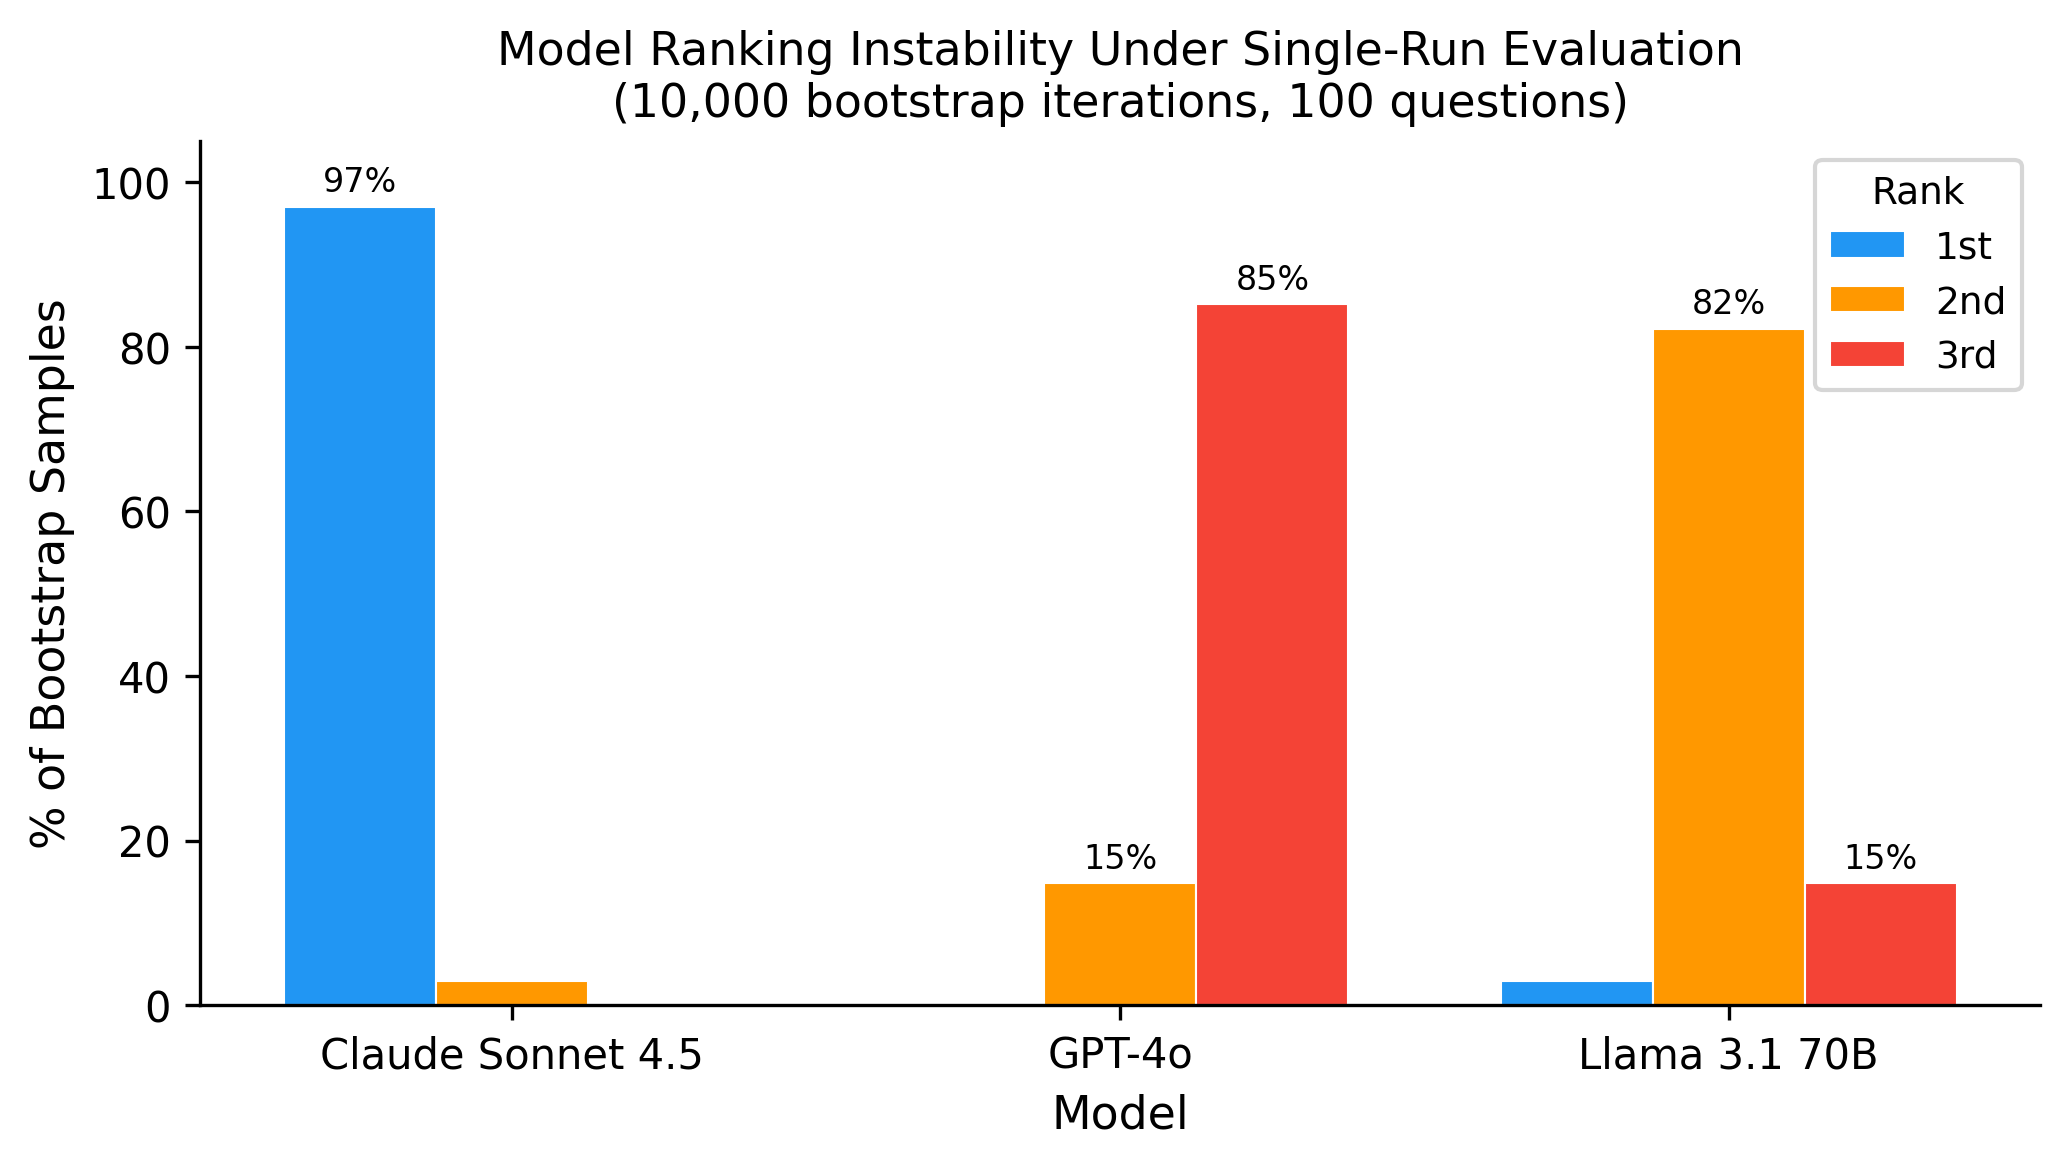
\includegraphics[width=\columnwidth]{rankings_instability.png}
\caption{Model ranking instability under single-run evaluation. In 17.8\% of bootstrap samples, the ranking differs from the multi-run ranking. The 2nd and 3rd positions (GPT-4o vs.\ Llama) are particularly unstable.}
\label{fig:rankings}
\end{figure}

Figure~\ref{fig:rankings} shows the results. Claude Sonnet 4.5 is robustly ranked 1st in 97.0\% of samples, but the 2nd and 3rd positions are unstable: Llama 3.1 70B and GPT-4o swap in 14.8\% of samples. Overall, \textbf{17.8\% of single-run evaluations produce a ranking that differs from the multi-run ground truth}. The instability stems from Llama's high variance: its single-run accuracy ranges from 67\% to 85\% (an 18pp spread), compared to Claude's 76--86\% (10pp) and GPT-4o's 67--79\% (12pp). In 3.0\% of samples, Llama even overtakes Claude for 1st place.

This has direct implications for benchmark methodology. When practitioners select models based on single-run leaderboard scores, they face nearly a 1-in-5 chance of obtaining the wrong ranking among these three models. The problem is worst for models with high behavioral variance, precisely the models whose single-run scores are least reliable. Agent evaluations should report multi-run statistics and confidence intervals; single-run accuracy is insufficient for reliable model comparison.

% ============================================================================
% DISCUSSION
% ============================================================================
\section{Discussion}

\paragraph{Differentiation from Prior Work.}
While $\tau$-bench \citep{yao2024tau} established that agents are inconsistent (pass$^k$ drops rapidly with $k$), our work provides complementary insights: (1) we identify \emph{where} variance originates (69\% at step 2), (2) we quantify the consistency-correctness relationship across three models (32--55pp gap), (3) we show path length predicts both consistency and correctness, and (4) we demonstrate that temperature is a key lever for controlling consistency. These findings suggest actionable interventions beyond simply measuring pass$^k$.

\paragraph{Consistency as a Runtime Signal.}
The strong correlation between consistency and correctness in this setting suggests a practical intervention: run multiple parallel executions and check for agreement. If runs diverge early, the answer is less likely to be correct. This could enable selective human review or automatic retry strategies.



\paragraph{The Step 2 Bottleneck.}
The concentration of divergence at step 2 suggests the first search query is critical. Improving query formulation, through better prompting, query expansion, or learned retrievers, could reduce downstream variance.

\paragraph{Implications for Complex Agents.}
Our study uses a minimal action space of three tools, yet we observe substantial behavioral variance. Our SWE-bench validation (Section~\ref{sec:swebench}) confirms that these patterns intensify with task complexity: accuracy gaps widen from 8pp (HotpotQA) to 54pp (SWE-bench) between the most and least consistent models, and 100\% of trajectories become unique. Since each action choice is a potential divergence point, consistency monitoring may be especially critical for capable, general-purpose agents deployed on complex tasks.

\paragraph{Model Selection.}
Our results suggest Claude Sonnet 4.5 may be preferable for applications requiring reliability, as it achieves both highest accuracy (81.9\%) and consistency (2.0 unique sequences). For open-source deployments, Llama 3.1 70B with reduced temperature (0.0--0.3) offers a reasonable alternative.

\paragraph{Capability and Consistency.}
The most capable model in our evaluation (Claude Sonnet 4.5) also exhibited the highest consistency, while the open-source model (Llama 3.1 70B) showed the most variance. This suggests a potential relationship between model capability and behavioral stability, though with only three models we cannot establish causality. Future work should investigate whether consistency improves predictably with scale or capability.

\paragraph{Implications for Benchmarking.}
Our ranking instability analysis (Section~\ref{sec:rankings}) reveals that single-run evaluations are fundamentally unreliable for comparing agent models. In 17.8\% of bootstrap samples, the model ranking differs from the multi-run ground truth. The most variable model (Llama 3.1 70B) has the least stable rank, ranging from 1st to 3rd across samples. This suggests that leaderboard positions based on single-run accuracy may be misleading, particularly for models with high behavioral variance. We recommend that agent benchmarks adopt multi-run evaluation with reported confidence intervals as standard practice.

\paragraph{Limitations.}
Our primary analysis uses HotpotQA with lexical search; our SWE-bench validation (Section~\ref{sec:swebench}) addresses the single-benchmark concern by confirming generalization to a substantially different domain. Remaining limitations include: (1) both benchmarks use a single domain per benchmark (QA paragraphs, astropy repository), (2) the temperature ablation uses a smaller sample (20 questions), and (3) we cannot establish causality between consistency and accuracy from observational data alone.

\paragraph{Future Work.}
Having validated generalization from HotpotQA to SWE-bench, we plan to extend this analysis along two further axes: (1) \textit{multimodality}, where visual grounding may either stabilize agent behavior through concrete observations or introduce additional variance from vision encoding; and (2) \textit{domain diversity}, as analytical reasoning tasks (FinQA, GAIA) and embodied environments (ALFWorld) may exhibit different consistency patterns than information retrieval or software engineering.

% ============================================================================
% CONCLUSION
% ============================================================================
\section{Conclusion}

We present a systematic study of behavioral consistency in LLM-based agents across three models on HotpotQA (3,000 runs) and SWE-bench (150 runs). Our key finding is that consistency predicts correctness: agents that behave consistently achieve 80--92\% accuracy, while inconsistent agents achieve only 25--60\%, a gap of 32--55 percentage points. This relationship generalizes across benchmarks: the same consistency hierarchy (Claude $>$ GPT $>$ Llama) holds on both simple QA and complex software engineering tasks, with accuracy gaps widening as task complexity increases. Moreover, single-run evaluations produce incorrect model rankings 17.8\% of the time, demonstrating that behavioral variance undermines standard benchmark methodology. Divergence occurs early (step 2), path length serves as a reliable signal, and reducing temperature improves both consistency and accuracy. These findings have practical implications for agent deployment: monitoring behavioral consistency could enable early error detection, and multi-run evaluation should replace single-run accuracy as the standard for agent benchmarks.


Code and data are available at \url{https://github.com/amanmehta-maniac/agent-consistency}.

% ============================================================================
% IMPACT STATEMENT
% ============================================================================
\section*{Impact Statement}

This paper presents work whose goal is to advance the field of machine learning. There are many potential societal consequences of our work, none of which we feel must be specifically highlighted here.

% ============================================================================
% REFERENCES
% ============================================================================
\bibliography{references}
\bibliographystyle{icml2026}

\end{document}
